\documentclass[t,aspectratio=169]{beamer} % 使用16:9宽高比
\usetheme{Madrid} % 选择Madrid主题
\usecolortheme{default} % 使用默认颜色主题

% 设置字体
\usepackage[UTF8]{ctex}
\usefonttheme{structurebold} % 加粗结构字体

% 数学包
\usepackage{amsmath, amssymb, bm}
\usepackage{url}
\usepackage{booktabs}

% 图形包
\usepackage{graphicx}

% 标题页信息
\title[10.5.图像分割]{第10章：卷积网络}
\subtitle{第5节：图像分割 (Image Segmentation)}
\author{《深度学习基础》课程小组}
% \institute{上海立信会计金融学院}
\date{\today}

\begin{document}

% 标题页
\frame{\titlepage}

% 目录页
\begin{frame}
    \frametitle{目录}
    \tableofcontents
\end{frame}

% ============================================================
% 第一部分：语义分割与卷积分割
% ============================================================
\section{语义分割与卷积分割}

\begin{frame}
    \frametitle{1. 语义分割 (10.5)}
    \begin{itemize}
        \item 图像分类：整图一个类别标签。
        \item 目标检测：多个物体 + 边界框。
        \item \alert{语义分割}：每个像素分配到预定义类别之一。
        \begin{itemize}
            \item 输出空间与输入图像\alert{同维度}
            \item 可方便地表示为相同像素数的图像
        \end{itemize}
        \item 输入图像：3 通道（R、G、B）。
        \item 输出数组：$C$ 通道（$C$ 个类别），表示各类别概率。
        \item 每类关联一种颜色，按最高概率着色。
    \end{itemize}
    \begin{figure}
        \centering
        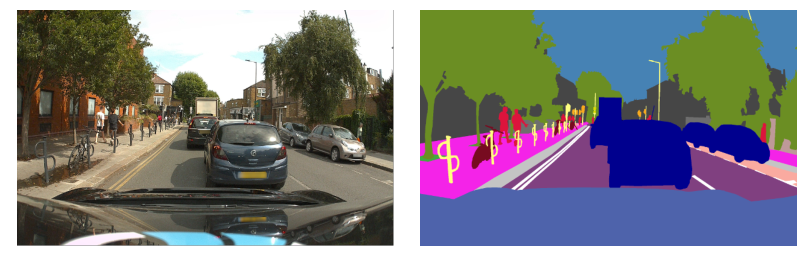
\includegraphics[width=0.4\textwidth]{ch10-5-1/figure-10-26.png}
        \caption{图像及其对应语义分割。}
    \end{figure}
\end{frame}

\begin{frame}
    \frametitle{1.1 卷积分割 (10.5.1)}
    \begin{itemize}
        \item \textbf{简单方法}：以每个像素为中心的矩形区域输入 CNN，单 softmax 输出分类该像素。
        \begin{itemize}
            \item 逐像素处理即可分割整张图像（需边缘填充）。
        \end{itemize}
        \item \textbf{问题}：重叠图像块导致\alert{大量冗余计算}，极其低效。
        \item \textbf{卷积化改进}：
        \begin{itemize}
            \item 将不同输入位置的前向传播计算组合到单个网络
            \item 最终全连接层也变为\alert{卷积层}
        \end{itemize}
        \item \textbf{保持维度}：每层步幅 1 + 相同填充 + 无池化。
        \item 每个输出单元共享 softmax 权重。
    \end{itemize}
    \begin{block}{计算成本问题}
        虽概念上可行，但达到高精度仍需\alert{多层多通道}，对合理分辨率图像成本过高。
    \end{block}
\end{frame}

% ============================================================
% 第二部分：上采样
% ============================================================
\section{上采样}

\begin{frame}
    \frametitle{2. 上采样 (10.5.2)}
    \begin{itemize}
        \item 大多数卷积网络使用\alert{下采样}：通道数增加时特征图尺寸减小。
        \begin{itemize}
            \item 保持网络规模和成本可控
            \item 提取高阶语义特征
        \end{itemize}
        \item \textbf{高效分割架构}：标准深度卷积网络 + \alert{可学习上采样层}。
        \begin{itemize}
            \item 将低维内部表示变换回原始图像分辨率
        \end{itemize}
    \end{itemize}
    \begin{figure}
        \centering
        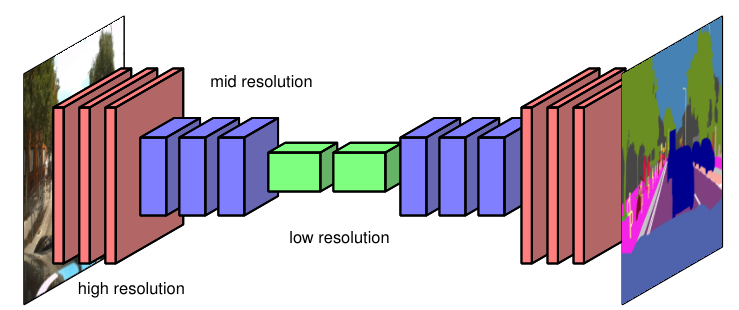
\includegraphics[width=0.45\textwidth]{ch10-5-2/figure-10-27.png}
        \caption{下采样（跨步卷积/池化）后跟上采样（转置卷积/反池化）。}
    \end{figure}
\end{frame}

\begin{frame}[allowframebreaks]
    \frametitle{2.1 反池化：池化的上采样对应}
    \begin{block}{平均池化的上采样对应}
        \begin{itemize}
            \item 将每个输入值\alert{复制到所有}对应的 $2 \times 2$ 输出单元
            \item 对输出应用平均池化可\alert{恢复输入}
        \end{itemize}
    \end{block}
    \begin{block}{最大池化的上采样对应（最大反池化）}
        \begin{itemize}
            \item 每个输入值复制到对应输出块的\alert{第一个单元}
            \item 其余值设为零
            \item 对输出应用最大池化可恢复输入
        \end{itemize}
    \end{block}
    \begin{figure}
        \centering
        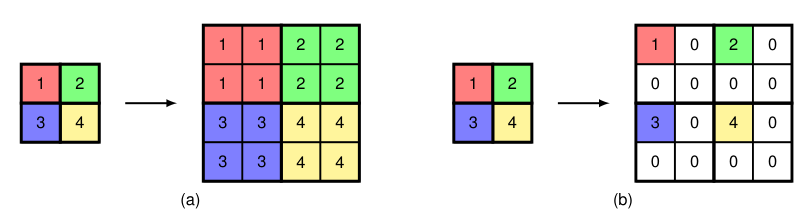
\includegraphics[width=0.5\textwidth]{ch10-5-2/figure-10-28.png}
        \caption{(a) 平均池化对应；(b) 最大池化对应。}
    \end{figure}
\end{frame}

\begin{frame}
    \frametitle{2.2 保留空间信息的改进方法}
    \begin{itemize}
        \item 将非零值固定在第一个元素\alert{过于随意}。
        \item \textbf{改进}：记录下采样时每个块中\alert{最大值的位置}。
        \item 上采样时将非零元素放在\alert{相同位置}。
        \item 保留更多来自下采样层的\alert{空间信息}。
    \end{itemize}
    \begin{figure}
        \centering
        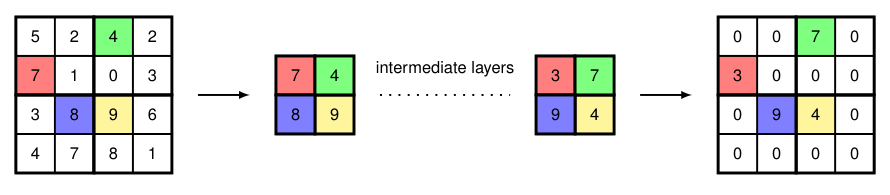
\includegraphics[width=0.55\textwidth]{ch10-5-2/figure-10-29.png}
        \caption{记录最大值位置，上采样时放在对应位置。}
    \end{figure}
\end{frame}

% ============================================================
% 第三部分：全卷积网络
% ============================================================
\section{全卷积网络}

\begin{frame}[allowframebreaks]
    \frametitle{3. 转置卷积 (10.5.3)}
    \begin{itemize}
        \item 固定上采样（反池化）之外，也可使用\alert{可学习上采样}。
        \item \textbf{跨步卷积（下采样）}：输出单元通过共享权重连接输入小块，输出维度低于输入。
        \item \textbf{转置卷积（上采样）}：输入一个像素连接到输出一个小块。
        \begin{itemize}
            \item 沿输入移动一步时，输出移动两步或更多步
            \item 输出维度高于输入
        \end{itemize}
        \item 重叠输出：对多个滤波器位置的贡献\alert{求和或取平均}。
    \end{itemize}
    \begin{figure}
        \centering
        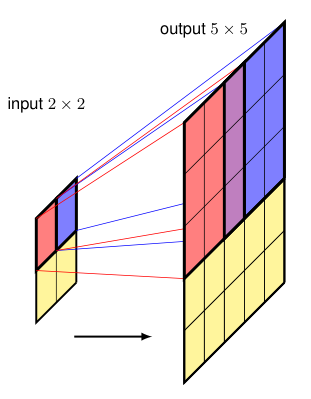
\includegraphics[width=0.25\textwidth]{ch10-5-3/figure-10-30.png}
        \caption{$3 \times 3$ 滤波器，输出步幅 2 的转置卷积。}
    \end{figure}
\end{frame}

\begin{frame}
    \frametitle{3.1 转置卷积的名称与全卷积网络}
    \begin{block}{名称来源}
        \begin{itemize}
            \item \alert{转置卷积}：下采样卷积写成矩阵后，上采样由\alert{转置矩阵}给出。
            \item \alert{分数步幅卷积}：步幅 = 输出步长 / 输入步长（图 10.30 中为 $1/2$）。
            \item \textbf{避免}用“反卷积”：数学中反卷积是泛函分析中卷积的逆，概念不同。
        \end{itemize}
    \end{block}
    \begin{block}{全卷积网络 (FCN)}
        \begin{itemize}
            \item 无池化层，下采样和上采样\alert{完全由卷积完成}。
            \item 可接受\alert{任意大小}的图像。
            \item 输出\alert{相同大小}的分割图。
        \end{itemize}
    \end{block}
\end{frame}

% ============================================================
% 第四部分：U-net 架构
% ============================================================
\section{U-net 架构}

\begin{frame}
    \frametitle{4. U-net 架构 (10.5.4)}
    \begin{itemize}
        \item 下采样允许增加通道数，但降低\alert{空间分辨率}，丢弃位置信息。
        \item 图像分类可容忍，但语义分割\alert{需要逐像素分类}。
        \item \alert{U-net} (Ronneberger et al., 2015)：解决空间信息丢失问题。
        \begin{itemize}
            \item 名称来自示意图的\alert{U 形}
        \end{itemize}
    \end{itemize}
    \begin{block}{核心结构}
        \begin{itemize}
            \item 对称排列的下采样层和上采样层
            \item 每个下采样层都有对应的上采样层
            \item 下采样层最终的通道激活与对应上采样层的\alert{第一组通道拼接}
            \item 通过拼接，上采样层可访问\alert{更高分辨率的空间信息}
        \end{itemize}
    \end{block}
    % \begin{figure}
    %     \centering
    %     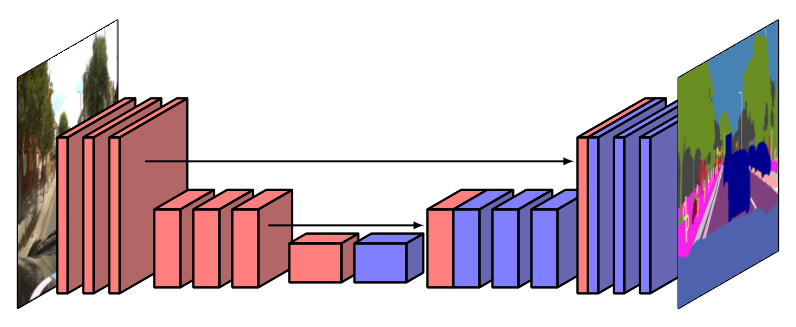
\includegraphics[width=0.45\textwidth]{ch10-5-4/figure-10-31.png}
    %     \caption{U-net 架构：对称下采样/上采样 + 拼接。}
    % \end{figure}
\end{frame}

\begin{frame}
    \frametitle{4.1 U-net 的最后一层}
    \begin{itemize}
        \item 最后一层可使用 $1 \times 1$ 卷积：
        \begin{itemize}
            \item 将通道数减少到\alert{类别数}
            \item 接 \alert{softmax} 激活函数
        \end{itemize}
        \item U-net 是一种\alert{全卷积网络}：
        \begin{itemize}
            \item 继承可接受任意大小输入、输出相同大小分割图的特性
        \end{itemize}
        \item 拼接 vs 相加：
        \begin{itemize}
            \item U-net 使用通道\alert{拼接}（concatenation），而非逐元素相加
            \item 拼接保留高分辨率信息
        \end{itemize}
    \end{itemize}
\end{frame}

% ============================================================
% 第五部分：总结
% ============================================================
\section{总结}

\begin{frame}[allowframebreaks]
    \frametitle{5. 本节总结}
    \begin{itemize}
        \item \alert{语义分割}：
        \begin{itemize}
            \item 每个像素分配到预定义类别
            \item 输出与输入同维度，$C$ 个通道
        \end{itemize}
        \item \alert{卷积分割}：
        \begin{itemize}
            \item 逐像素 CNN 冗余计算
            \item 卷积化改进：全连接层卷积化
            \item 保持维度：步幅 1 + 相同填充 + 无池化
        \end{itemize}
        \item \alert{上采样}：
        \begin{itemize}
            \item 反池化：平均池化对应（复制到块） / 最大池化对应（放在块首）
            \item 改进：记录最大值位置，上采样时放在相同位置
        \end{itemize}
        \item \alert{转置卷积}：
        \begin{itemize}
            \item 下采样卷积的转置矩阵
            \item 分数步幅卷积
            \item 避免用“反卷积”一词
        \end{itemize}
        \item \alert{全卷积网络}：无池化，完全由卷积完成，任意输入大小。
        \item \alert{U-net}：
        \begin{itemize}
            \item 对称下采样/上采样 + 跳跃拼接
            \item 最后一层 $1 \times 1$ 卷积 + softmax
            \item 同时获得语义与空间信息
        \end{itemize}
    \end{itemize}
\end{frame}

% ============================================================
% 第六部分：参考文献
% ============================================================
\section{参考文献}

\begin{frame}
    \frametitle{6. 参考文献}
    \begin{itemize}
        \item 教材：Bishop, C. M. \& Bishop, H. (2023). Deep Learning Foundations and Concepts. Springer Nature Switzerland AG.
        \item Long, J., Shelhamer, E., \& Darrell, T. (2014). Fully convolutional networks for semantic segmentation.
        \item Noh, H., Hong, S., \& Han, B. (2015). Learning deconvolution network for semantic segmentation.
        \item Badrinarayanan, V., Kendall, A., \& Cipolla, R. (2015). SegNet: A deep convolutional encoder-decoder architecture.
        \item Ronneberger, O., Fischer, P., \& Brox, T. (2015). U-Net: Convolutional networks for biomedical image segmentation.
        \item Dumoulin, V. \& Visin, F. (2016). A guide to convolution arithmetic for deep learning.
    \end{itemize}
\end{frame}

\end{document}